%%%%%%%%%%%%%%%%%%%%%%%%%%%%%%%%%%%%
% Slide options
%%%%%%%%%%%%%%%%%%%%%%%%%%%%%%%%%%%%

% Option 1: Slides with solutions

\documentclass[slidestop,compress,mathserif]{beamer}
\newcommand{\soln}[1]{\textit{#1}}
\newcommand{\solnGr}[1]{#1}

% Option 2: Handouts without solutions

%\documentclass[11pt,containsverbatim,handout]{beamer}
%\usepackage{pgfpages}
%\pgfpagesuselayout{4 on 1}[letterpaper,landscape,border shrink=5mm]
%\newcommand{\soln}[1]{ }
%\newcommand{\solnGr}{ }

%%%%%%%%%%%%%%%%%%%%%%%%%%%%%%%%%%%%
% Style
%%%%%%%%%%%%%%%%%%%%%%%%%%%%%%%%%%%%
\def\chp8@path{../../Chp 8}
\input{../../lec_style.tex}


%%%%%%%%%%%%%%%%%%%%%%%%%%%%%%%%%%%%
% Preamble
%%%%%%%%%%%%%%%%%%%%%%%%%%%%%%%%%%%%

\title[Lecture 31]{MA213: Lecture 31}
\subtitle{Module 5: Linear regression}
\author{OpenIntro Statistics, 4th Edition}
\institute{$\:$ \\ {\footnotesize Based on slides developed by Mine \c{C}etinkaya-Rundel of OpenIntro. \\
The slides may be copied, edited, and/or shared via the \webLink{http://creativecommons.org/licenses/by-sa/3.0/us/}{CC BY-SA license.} \\
Some images may be included under fair use guidelines (educational purposes).}}
\date{}


%%%%%%%%%%%%%%%%%%%%%%%%%%%%%%%%%%%%
% Begin document
%%%%%%%%%%%%%%%%%%%%%%%%%%%%%%%%%%%%

\begin{document}


%%%%%%%%%%%%%%%%%%%%%%%%%%%%%%%%%%%%
% Title page
%%%%%%%%%%%%%%%%%%%%%%%%%%%%%%%%%%%%

{
\addtocounter{framenumber}{-1} 
{\removepagenumbers 
\usebackgroundtemplate{\includegraphics[width=\paperwidth]{../../OpenIntro_Grid_4_3-01.jpg}}
\begin{frame}

\hfill \includegraphics[width=20mm]{../../oiLogo_highres}

\titlepage

\end{frame}
}
}


%%%%%%%%%%%%%%%%%%%%%%%%%%%%%%%%%%%%
% Recap/Agenda 
%%%%%%%%%%%%%%%%%%%%%%%%%%%%%%%%%%%%
% TODO better formatting
\begin{frame}
    \frametitle{Module 4: Inference}
    \begin{itemize}
        \item \hl{Previously: }Comparing many means with ANOVA (Chapter 7.5)
        \item \hl{This time: }Issues with Hypothesis Testing 2: Multiple comparisons
        \item \hl{Reading: }Chapter 8.1 for next time
        \item \hl{Deadlines/Announcements: }HW 4.3 due Monday
    \end{itemize}
    
\end{frame}
%%%%%%%%%%%%%%%%%%%%%%%%%%%%%%%%%%%%
% Sections
%%%%%%%%%%%%%%%%%%%%%%%%%%%%%%%%%%%%

%%%%%%%%%%%%%%%%%%%%%%%%%%%%%%%%%%%%

\section{Line fitting, residuals, and correlation}

%%%%%%%%%%%%%%%%%%%%%%%%%%%%%%%%%%%%

\subsection{Fitting a line to data}

%%%%%%%%%%%%%%%%%%%%%%%%%%%%%%%%%%%%

\begin{frame}
\frametitle{Modeling numerical variables}

In this unit we will learn to quantify the relationship between two numerical variables, as well as modeling numerical response variables using a numerical or categorical explanatory variable.

\end{frame}

%%%%%%%%%%%%%%%%%%%%%%%%%%%%%%%%%%%%
\section{R Demonstration: Scatterplots and associations}
%%%%%%%%%%%%%%%%%%%%%%%%%%%%%%%%%%%%

\begin{frame}
\frametitle{Poverty vs. HS graduate rate}

The \hl{scatterplot} below shows the relationship between HS graduate rate in all 50 US states and DC and the \% of residents who live below the poverty line {\small (income below \$23,050 for a family of 4 in 2012)}.

\twocol{0.55}{0.45}{
\begin{center}
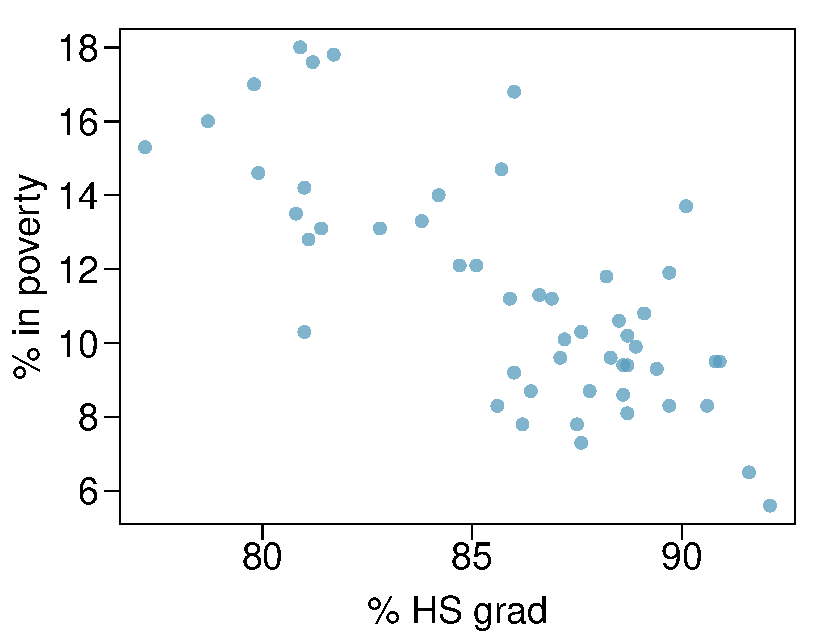
\includegraphics[width=\textwidth]{\chp8@path/8-1_linefit_res_corr/figures/poverty/poverty_hsgrad}
\end{center}
}
{
\dq{Response variable?}
\pause
\soln{\% in poverty}
\pause
\dq{Explanatory variable?}
\pause
\soln{\% HS grad}
\pause
\dq{Relationship?}
\pause
\soln{linear, negative, moderately strong}
}

\end{frame}

%%%%%%%%%%%%%%%%%%%%%%%%%%%%%%%%%%%

\section{Edfinity Quiz: Defining relationships practice}

%%%%%%%%%%%%%%%%%%%%%%%%%%%%%%%%%%%

\subsection{Using a linear regression to predict poverty}

%%%%%%%%%%%%%%%%%%%%%%%%%%%%%%%%%%%

\begin{frame}

The linear model for predicting poverty from high school graduation rate in the US is

\[ \hat{poverty} = 64.78 - 0.62 * HS_{grad} \]

The ``hat" is used to signify that this is an estimate.

\end{frame}

%%%%%%%%%%%%%%%%%%%%%%%%%%%%%%%%%%%

\begin{frame}

\dq{The high school graduate rate in Georgia is 85.1\%. What poverty level does the model predict for this state?}

\pause

\[ 64.78 - 0.62 * 85.1 = 12.018 \]

\end{frame}

%%%%%%%%%%%%%%%%%%%%%%%%%%%%%%%%%%%

\subsection{Eyeballing the line}

%%%%%%%%%%%%%%%%%%%%%%%%%%%%%%%%%%%

\begin{frame}
\frametitle{Eyeballing the line}

\twocol{0.3}{0.7}
{
\pq{Which of the following appears to be the line that best fits the linear relationship between \% in poverty and \% HS grad? Choose one.}
\soln{\only<2>{\orange{
(a)
}}}
}
{
\begin{center}
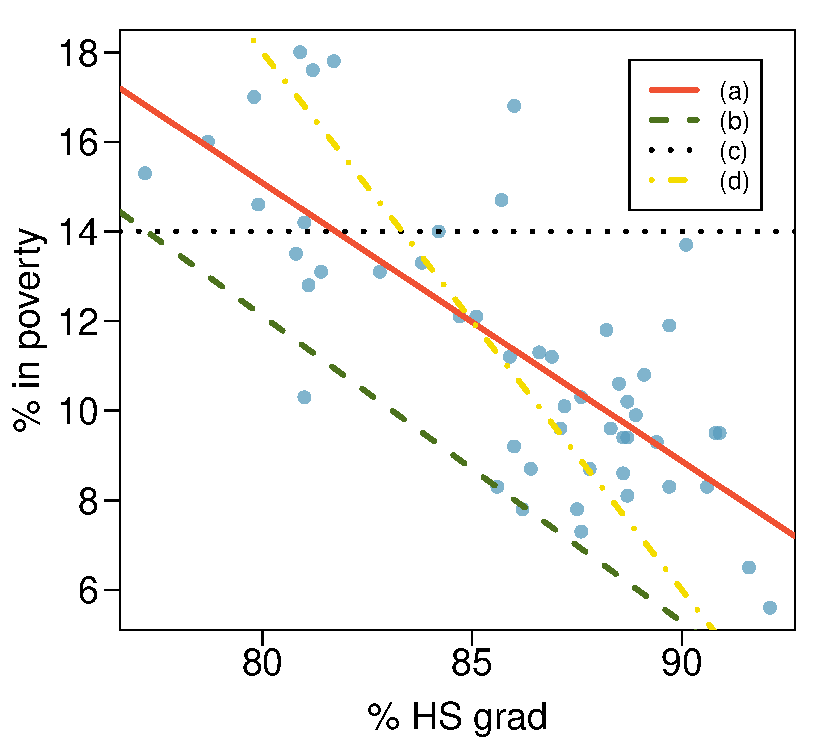
\includegraphics[width=\textwidth]{\chp8@path/8-2_least_square_reg/figures/poverty/poverty_hsgrad_manylines}
\end{center}
}
\end{frame}

%%%%%%%%%%%%%%%%%%%%%%%%%%%%%%%%%%%

\subsection{Residuals}

%%%%%%%%%%%%%%%%%%%%%%%%%%%%%%%%%%%

\begin{frame}
\frametitle{Residuals}

\hl{Residuals} are the leftovers from the model fit: Data = Fit + Residual

\begin{center}
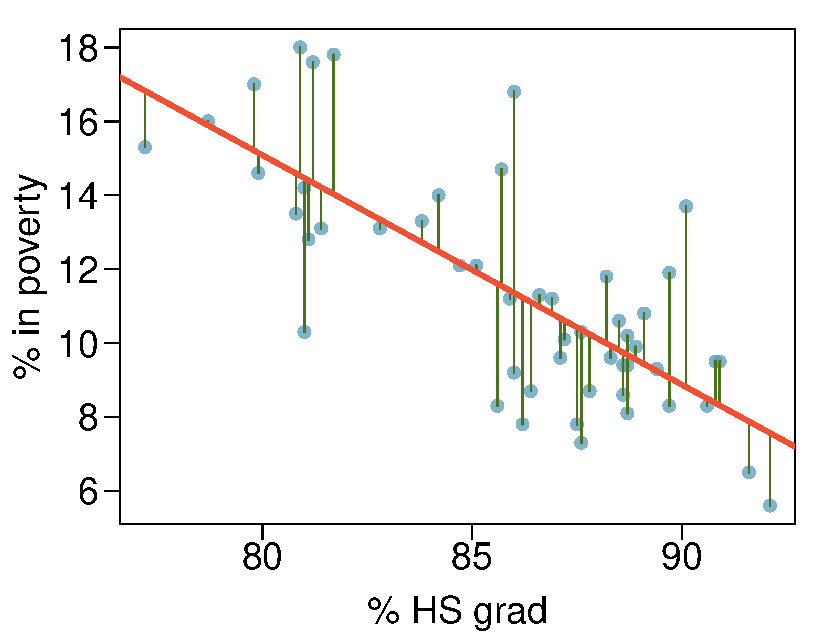
\includegraphics[width=0.8\textwidth]{\chp8@path/8-2_least_square_reg/figures/poverty/poverty_hsgrad_res}
\end{center}

\end{frame}

%%%%%%%%%%%%%%%%%%%%%%%%%%%%%%%%%%

\begin{frame}
\frametitle{Residuals (cont.)}

\formula{Residual}{
Residual is the difference between the observed ($y_i$) and predicted $\hat{y}_i$. 
\[ e_i = y_i - \hat{y}_i \]
}
\vspace{-0.5cm}
\twocol{0.6}{0.4}
{
\begin{center}
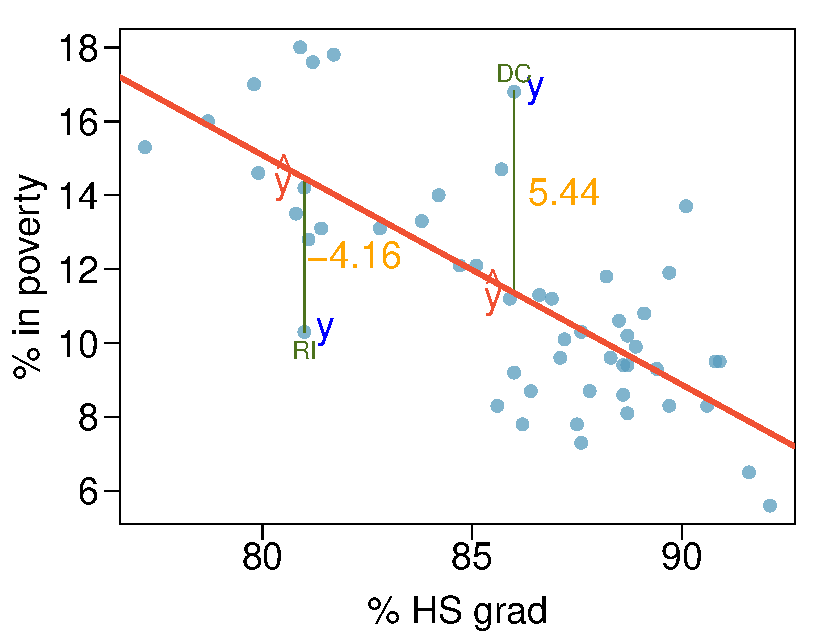
\includegraphics[width=\textwidth]{\chp8@path/8-2_least_square_reg/figures/poverty/poverty_hsgrad_res_text}
\end{center}
}
{
\pause
\begin{itemize}
\item \% living in poverty in DC is 5.44\% more than predicted.
\pause
\item \% living in poverty in RI is 4.16\% less than predicted.
\end{itemize}
}


\end{frame}

%%%%%%%%%%%%%%%%%%%%%%%%%%%%%%%%%%

\subsection{Describing linear relationships with correlation}

%%%%%%%%%%%%%%%%%%%%%%%%%%%%%%%%%%%

\begin{frame}
\frametitle{Quantifying the relationship}

\begin{itemize}

\item \hl{Correlation} describes the strength of the \orange{linear} association between two variables.

\pause

\item It takes values between -1 (perfect negative) and +1 (perfect positive).

\pause

\item A value of 0 indicates no linear association.

\end{itemize}

\end{frame}

%%%%%%%%%%%%%%%%%%%%%%%%%%%%%%%%%%%

\section{Edfinity Quiz: Correlation}

%%%%%%%%%%%%%%%%%%%%%%%%%%%%%%%%%%%

\begin{frame}
\frametitle{Guessing the correlation}

\pq{Which of the following is the best guess for the correlation between \% in poverty and \% HS grad?}
\twocol{0.4}{0.6}
{
\begin{enumerate}[(a)]
\item 0.6
\solnMult{-0.75}
\item -0.1
\item 0.02
\item -1.5
\end{enumerate}
}
{
\begin{center}
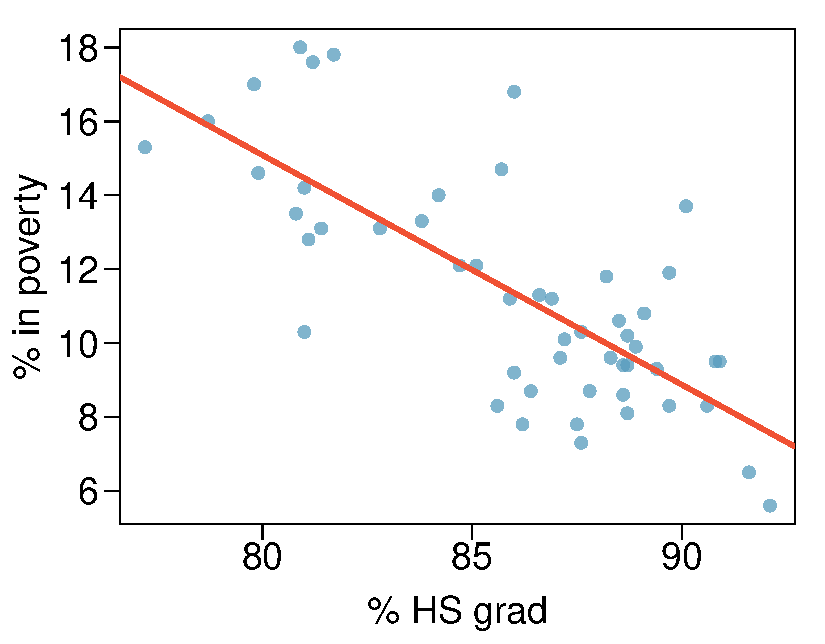
\includegraphics[width=\textwidth]{\chp8@path/8-1_linefit_res_corr/figures/poverty/poverty_hsgrad_line}
\end{center}
}

\end{frame}

%%%%%%%%%%%%%%%%%%%%%%%%%%%%%%%%%%

\begin{frame}
\frametitle{Guessing the correlation}

\pq{Which of the following is the best guess for the correlation between \%~in~poverty and \%~female~householder,~no~husband~present?}

\twocol{0.4}{0.6}
{
\begin{enumerate}[(a)]
\item 0.1
\item -0.6
\item -0.4
\item 0.9
\solnMult{0.5}
\end{enumerate}
}
{
\begin{center}
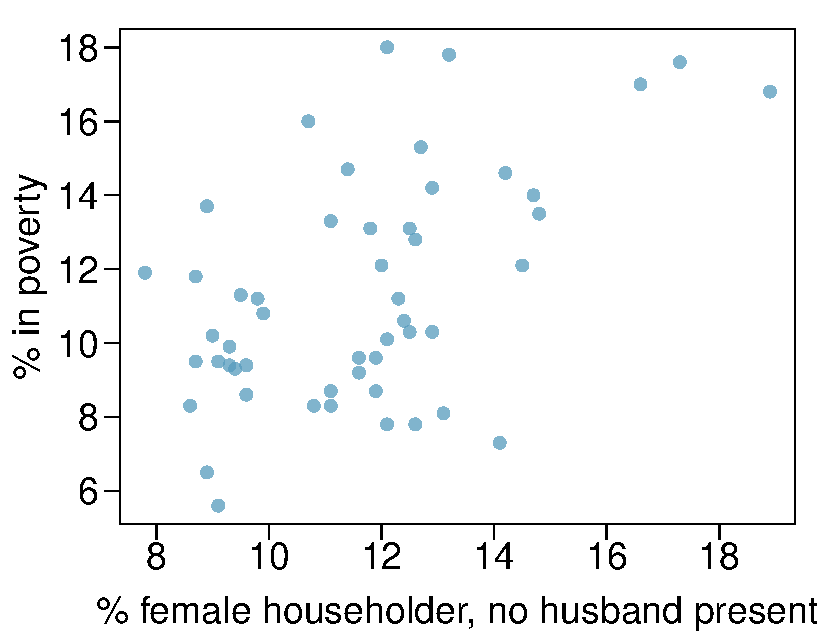
\includegraphics[width=\textwidth]{\chp8@path/8-1_linefit_res_corr/figures/poverty/poverty_nohusband}
\end{center}
}

\end{frame}

%%%%%%%%%%%%%%%%%%%%%%%%%%%%%%%%%%

\begin{frame}
\frametitle{Assessing the correlation}

\pq{Which of the following is has the strongest correlation, i.e. correlation coefficient closest to +1 or -1?}

\twocol{0.8}{0.2}
{
\begin{center}
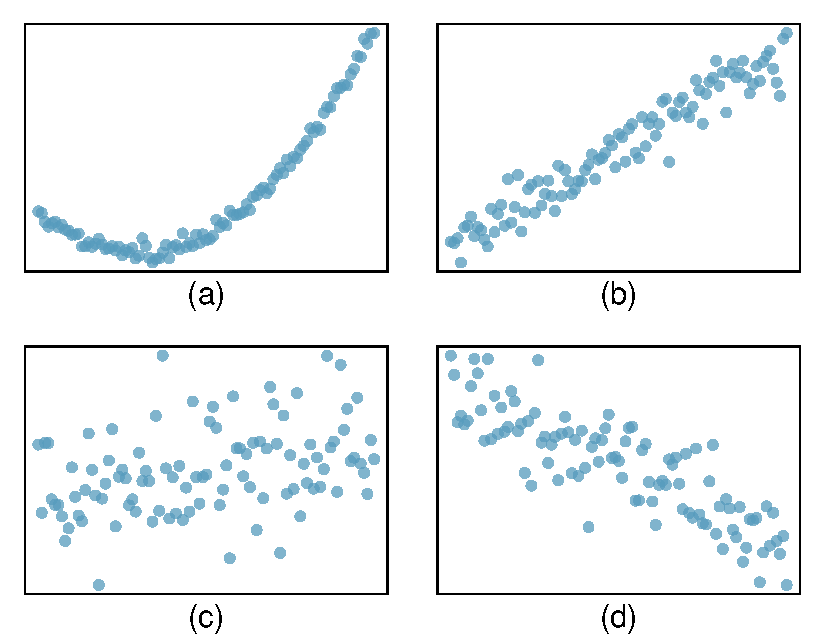
\includegraphics[width=0.75\textwidth]{\chp8@path/8-1_linefit_res_corr/figures/cor/cor}
\end{center}
}
{
\soln{\only<2>{\orange{
(b) $\rightarrow$ correlation means \underline{linear} association
}}}
}

\end{frame}

%%%%%%%%%%%%%%%%%%%%%%%%%%%%%%%%%%

\section{Preview to line-fitting}

\begin{frame}
    \frametitle{Motivation}
\end{frame}

%%%%%%%%%%%%%%%%%%%%%%%%%%%%%%%%%%%%
% End document
%%%%%%%%%%%%%%%%%%%%%%%%%%%%%%%%%%%%

\end{document}